\section{Introduction to Limits: The Motivation}

\begin{idea}
    The goal of the first few lectures is to define the derivative of a function \textit{rigorously} \textbf{logically}. There are similar, but not quite the same, problems to the above:
    \begin{itemize}
        \item Defining the \emph{slope} of a tangent to the curve
        \item Defining \emph{speed} at an \textit{instant}.
    \end{itemize}
    However, these concepts are not very well defined.
\end{idea}
\begin{itemize}
    \item Consider a falling object where a ball starts at a height of $d=0$ and ends at a distance of $d(t)$.
    \begin{center}
        \begin{tikzpicture}[x=1cm,y=1cm]
            \draw[semithick] (-2,4) -- (0,4) -- (0,0) -- (5,0);
            
            \draw[fill=black] (1,1) circle (0.1);
            
            \draw[<-,thick] (2,3) -- (3,3) node [midway, below] {$\bm{d}=0$};
            \draw[<-,thick] (2,1) -- (3,1) node [midway, below] {$\bm{d}(t)$};

            \draw[->,thick] (4,3) -- (4,1) node [midway, right] {$\bm{d}$};
        \end{tikzpicture}
    \end{center}
    Suppose we are given the function $d(t)=5t^2$ where $d$ is in meters and $t$ is in seconds.
    % \begin{center}
    %     \begin{tikzpicture}
    %     \begin{axis}[
    %     legend pos=south east,
    %     title=Plot of $d(t)$,
    %     axis lines = box,
    %     grid = both,
    %     axis lines = middle,
    %     xlabel = $t$,
    %     ylabel = $d(t)$,
    %     variable = t,
    %     trig format plots = rad,
    %     ]
    %     \addplot [
    %         domain=0:2,
    %         samples=70,
    %         color=blue,
    %         ]
    %         {x*x};
    %     \end{axis}
    %     \end{tikzpicture}
    % \end{center}
    To determine the speed at the \emph{instant} $t=1 \text{ sec}$, we can approximate using a secant-line:
    \begin{align}
        m_\text{sec} &= \frac{5(1.1)^2-5(1)^2}{1.1-1}=10.5 \text{ m/s} \\ 
        m_\text{sec} &= \frac{5(1.01)^2-5(1)^2}{1.01-1}=10.05 \text{ m/s} 
        \label{eq:}
    \end{align}
    The instantaneous speed \textit{appears} to approach $10 \text{ m/s}$ \textbf{exactly} at $t=1 \text{ sec}$, but we \emph{cannot} be sure. \item We can do better by introducing a new variable $x[s]$ which represents the interval:
    \begin{center}
        \begin{tikzpicture}
            \begin{axis}[
                axis x line=center, 
                axis y line=middle, 
                xtick={0,1,1.4},
                xticklabels={$0$,$1$,$1+x$},
                ytick={5,9.8},
                yticklabels={$5$,$d(1+x)$},
                domain=0:2,
                xlabel = $t$,
                ylabel = $d(t)$,
            ]
            \addplot[samples=70,color=blue] {5*x*x};
            \addplot[domain=0.6:1.8,samples=70,color=blue] {12*x-7};

            \node[circle,color=blue,fill,inner sep=2pt] at (axis cs:1,5) {};
            \node[circle,color=blue,fill,inner sep=2pt] at (axis cs:1.4,9.8) {};
            \draw[dashed] (1,0) -- (1,5);
            \draw[dashed] (1.4,0) -- (1.4,9.8);
            \draw[dashed] (0,5) -- (1,5);
            \draw[dashed] (0,9.8) -- (1.4,9.8);
            \end{axis}
        \end{tikzpicture}
    \end{center}
    We then define a function $f(x)$ as
    \begin{align}
        f(x) &\equiv \frac{d(1+x)-d(1)}{x} \\ 
        &= \frac{5(1+x)^2-5(1)^2}{x} \\ 
        &= \frac{10x+5x^2}{x} \\ 
        &= (10+5x)\left(\frac{x}{x}\right)
    \end{align}
    Let us \textit{assume} (incorrectly) that $\frac{x}{x}=1$ for all $x$. Then:
    \begin{equation}
        f(x) = 10x+5
        \label{eq:}
    \end{equation}
    So we could define the ``speed at $t=1 \text{ s}$'' as $f(0)$ which is exactly $10$.
    \begin{warning}
        However: $\frac{x}{x} \neq 1$ when $x=0$ as division by zero is not allowed as a legitimate operation of arithmetic. To explain why, we need to rigorously introduce numbers as defined by \textbf{axioms}.
        \begin{itemize}
            \item Example: For every $x\neq 0$
            there is another number $\frac{1}{x}$ defined \textbf{implicitly} by $x \cdot \frac{1}{x} =1$.
        \end{itemize}
        \vspace{2mm}

        An implicit definition is when a quantity we are defining does not appear by itself on one side of the equation. Implicit definitions are used for the most basic axioms. If this was not true, then we can contradict ourselves. We would have:
        \begin{equation}
            0 \cdot \frac{1}{0} = 1
            \label{eq:}
        \end{equation}
        but we can also prove that $0\cdot a=0$ for all numbers $a$, so if $\frac{1}{0}$ is a number, then $0=1$.
        \vspace{2mm}

        Furthermore, it is not possible to define $\frac{1}{0}$ if it was a number. A naive approach may be to define it as infinity, but infinity is not a number! If it was, then:
        \begin{align}
            1+\infty &= \infty \\ 
            2+\infty &= \infty \\ 
            1 &= 2
        \end{align}
        Just because you \textbf{write} some symbol does not mean it \textbf{exists} as a number.
    \end{warning}
    The correct expression for $f(x)$ is instead:
    \begin{equation}
        f(x) = \begin{cases}10+5x, & x\neq 0 \\ \text{DNE}, & x=0\end{cases}
        \label{eq:10x+5x^2}
    \end{equation}
    While $\text{DNE}$ is not a number, $f(x)$ is still a legitimate function. We don't \textit{fix} functions.
    \item The \textbf{limit} can be used to satisfy our intuitive feeling that the answer is exactly $10 \text{ m/s}$. The expression:
    \begin{equation}
        \lim_{x\to 0}f(x)
        \label{eq:}
    \end{equation}
    is a number.
    \begin{warning}
        We can't always trust our intuition on whether a certain relationship will converge or diverge:
        \begin{align}
            A &= \frac{1}{2}+\frac{1}{4}+\frac{1}{8}+\frac{1}{17}+\cdots \\ 
            B &= \frac{1}{2}+\frac{1}{3}+\frac{1}{4}+\frac{1}{5} + \cdots
        \end{align}
        The value of $A$ will converge to $1$, but the value of $B$ will diverge\footnote{This is known as the harmonic sum.} and will not exist. This is why we need a rigorous definition of what exactly ``approaching'' means.
    \end{warning}
    \item A simpler type of limit considers what happens at infinity:
    \begin{center}
        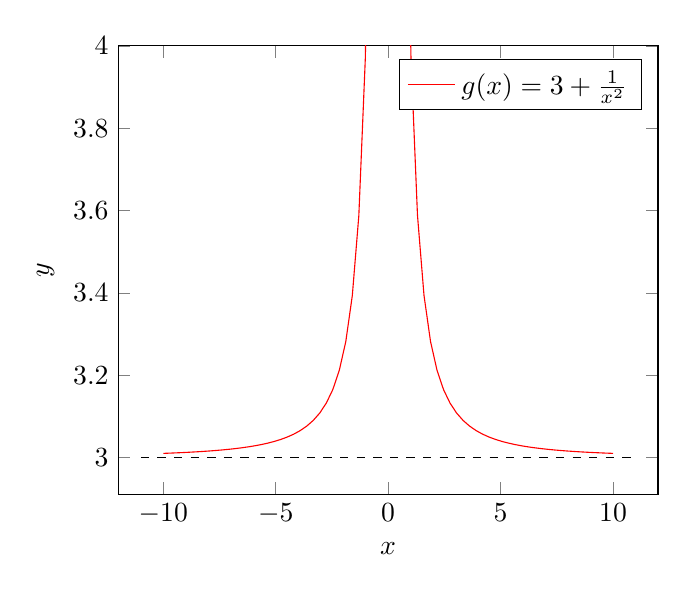
\begin{tikzpicture}
        \begin{axis}[
        legend pos=north east,
        axis lines = box,
        xlabel = $x$,
        ylabel = $y$,
        ymax = 4,
        variable = t,
        trig format plots = rad,
        ]
        \addplot [
            domain=-10:10,
            samples=70,
            color=red,
            ]
            {3 + 1/(x*x)};
        \addlegendentry{$g(x)=3+\frac{1}{x^2}$}
        
        \draw[dashed] (-11,3) -- (11,3);
        \end{axis}
        \end{tikzpicture}
    \end{center}
    It appears that $g(x)$ approaches a value of $3$ as $x$ approaches infinity. The challenge is to find a \textbf{rigorous definition} of:
    \begin{equation}
        \lim_{x\to\infty}g(x)
        \label{eq:}
    \end{equation}
    so that we can prove it exists as a number. We want to be able to say that we can always find values of $x$ large enough that the values of $g(x)$ will be as close as might be wanted to $3$, say within $10^{-10}$ of $3$. Geometrically, this is represented by always being able to pick an $x$ great enough such that $g(x)$ is contained within the dashed lines. 
    \begin{center}
        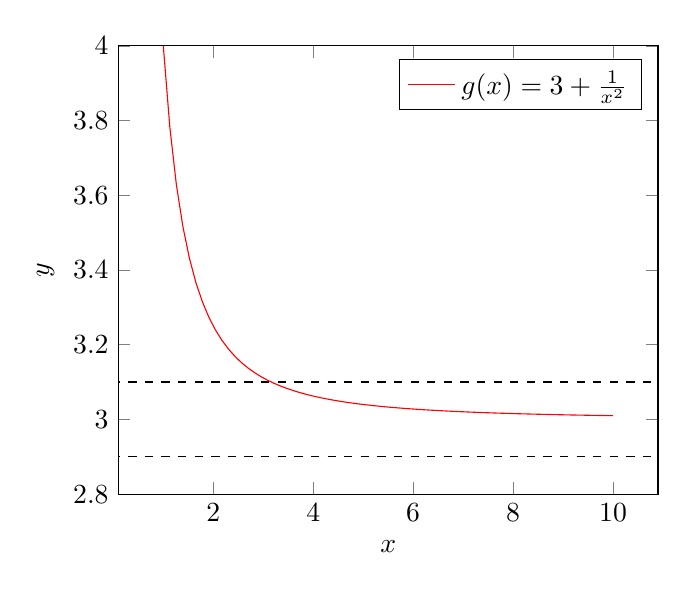
\begin{tikzpicture}
        \begin{axis}[
        legend pos=north east,
        axis lines = box,
        xlabel = $x$,
        ylabel = $y$,
        ymax = 4,
        ymin = 2.8,
        variable = t,
        trig format plots = rad,
        ]
        \addplot [
            domain=1:10,
            samples=70,
            color=red,
            ]
            {3 + 1/(x*x)};
        \addlegendentry{$g(x)=3+\frac{1}{x^2}$}
        \draw[dashed] (-11,3.1) -- (11,3.1);
        \draw[dashed] (-11,2.9) -- (11,2.9);
        \end{axis}
        \end{tikzpicture}
    \end{center}
    We can solve this via trial and error. Say for a large $x_0=10^{100}$, we can show that for all
    \begin{align}
        x &> x_0=10^{100} \\
        x^2 &> 10^{200} \\ 
        \frac{1}{x^2} &< 10^{-200} \\ 
        3+\frac{1}{x^2} &< 3+10^{-200}
    \end{align}
    Since $3+10^{-200}<3+10^{-10}$, then the weaker case:
    \begin{equation}
        g(x) < 3+10^{-10}
        \label{eq:}
    \end{equation}
    must be true for all $x>x_0=10^{100}$ However, we need to find the lower bound as well. Next, note that:
    \begin{equation}
        g(x)=3+\frac{1}{x^2} > 3 > 3-10^{-10}
        \label{eq:}
    \end{equation}
    for all $x$. Therefore, for all $x>10^{100}$, then:
    $3-10^{-10} < g(x) < 3+10^{-10}$.
    \item We can generalize this to any arbitrary bound. Some small number $\epsilon>0$. We want to find some $x_0$ expressed in terms of $\epsilon$ such that for all $x>x_0$, the values of $g(x)$ will be within $\epsilon$ of 3.
    \begin{mnemonic}
        The value of $\epsilon$ is imposed by the $\epsilon$nemy as a challenge.
    \end{mnemonic}
    Again, we use trial and error.
    \begin{example}
        Suppose we pick $x_0=\frac{1}{\epsilon}$. Then for all $x>x_0=\frac{1}{\epsilon}$, we have:
        \begin{align}
            x^2 &> \frac{1}{\epsilon^2} \\
            \frac{1}{x^2} &< \epsilon^2 \\ 
            3+\frac{1}{x^2} &< 3+\epsilon^2 \\ 
            g(x) &< 3+\epsilon^2 \\
        \end{align}
        which doesn't quite work since in order for the value to be within the bounds, the following must be true:
        \begin{equation}
            g(x) < 3+\epsilon^2 \le 3+ \epsilon
            \label{eq:}
        \end{equation}
        which is only true for $\epsilon \le 1$ and is not true for all values of $\epsilon$.
    \end{example}
    \begin{example}
        Suppose we pick $x_0=\frac{1}{\sqrt{\epsilon}}$. Then for all $x>x_0=\frac{1}{\sqrt\epsilon}$, we have:
        \begin{align}
            x^2 &> \frac{1}{\epsilon} \\
            \frac{1}{x^2} &< \epsilon \\ 
            3+\frac{1}{x^2} &< 3+\epsilon \\ 
            g(x) &< 3+\epsilon \\
        \end{align}
        which provides the correct upper bound!
    \end{example}
    As a result, the value of $y=3$ passes this challenge test, so we can define a new number:
    \begin{equation}
        \lim_{x\to\infty}g(x)
        \label{eq:}
    \end{equation}
    and assign it to the value of $3$.
    \begin{idea}
        There are three steps to find the limit:
        \begin{enumerate}
            \item Assume that $\displaystyle \lim_{x\to\infty}$ exists and guess a value for it.
            \item Show that your guess passes a ``challenge'' imposed by $\epsilon$
            \item If you succeed then we can take that $\displaystyle\lim_{x\to\infty}g(x)$ exists as a number since we can assign it to your original guess.
        \end{enumerate}
    \end{idea}
    \item Similarly, for our original function $f(x)$ we can use a similar way to define the limit as $x\to 0$.but 
\end{itemize}